\documentclass{beamer}
\mode<presentation>

\usepackage{amsmath}
\DeclareMathOperator*{\argmin}{\arg\!\min}

\usetheme{Singapore}
\title{Distributed Dual Averaging in Networks}
\subtitle{Project Presentation}
\author{Maxim Timchenko}
\institute{Electrical and Computer Engineering Department\\Boston University}
\date{EC 719 Statistical Pattern Recognition, Fall 2014}
\begin{document}
	\begin{frame}
		\titlepage
	\end{frame}
	
	\begin{frame}{Outline}
		\tableofcontents
	\end{frame}
	
	\section{The Problem}
	\begin{frame}{Problem Statement}
		\begin{description}
  			\item[Decentralized optimization]\hfill \\ Optimize a global objective
			formed by a sum of convex functions using local computation
			and local communication over a network of compute nodes.
			\pause
			\item[Theoretical performance] \hfill \\ Provide bounds on algorithm 
			convergence rates as function of network size and topology.
		\end{description}
	\end{frame}
	
	\section{Motivation}
	\begin{frame}{Motivation: Big Data}
		Classical ML: minimize a loss function over a dataset.\\
		Interesting datasets grow in size faster than innovations in 
		storage capacity of a single computer.
		\begin{itemize}
			\item Google Maps dataset in 2012: 20 PB (20,500 TB)\footnote{http://mashable.com/2012/08/22/google-maps-facts/}
			\item Facebook dataset in 2010: 20 PB, in 2011: 30 PB\footnote{https://www.facebook.com/notes/paul-yang/moving-an-elephant-large-scale-hadoop-data-migration-at-facebook/10150246275318920}
		\end{itemize}
		Non-ML distributed convex minimization: 
		multi-agent coordination, estimation in sensor networks,
		packet routing...
	\end{frame}	

	\begin{frame}{Motivation: Distributed Computation Constraints}
		In datacenter environments, supercomputers, and ad-hoc
		distributed networks, available bandwidth of communication 
		is in inverse relationship to distance.
		\begin{quote}Traditionally, inter-cluster connectivity is oversubscribed, with much less bandwidth available between the clusters than within them. This assumes and then dictates that most intra-application communications occur inside the cluster."\footnote{https://code.facebook.com/posts/360346274145943/introducing-data-center-fabric-the-next-generation-facebook-data-center-network/}\end{quote}
		
		Modelling the network as a graph with nearby connections as
		edges is convenient.
	\end{frame}
	
	\section{Related Work}
	\begin{frame}{Related Work}
		\begin{itemize}
			\item N. Tsitsiklis, D. P. Bertsekas, and M. Athans. 1986.
Distributed asynchronous deterministic and stochastic
gradient optimization algorithms. \emph{Uses shared memory.}
			\item D. P. Bertsekas, J. N. Tsitsiklis. Parallel and Distributed Computation: Numerical Methods. 1989.
			\item A. Nedic and A. Ozdaglar. Distributed subgradient methods for multi-agent optimization. 2009.\\ 
			\emph{Each agent has its own objective function.}
			\item Y. Nesterov. Primal-dual subgradient methods for convex problems. 2009. \\
			\emph{Non-distributed version of the proposed algorithm.}
		\end{itemize}
	\end{frame}
	
	\section{Contribution}
	\begin{frame}{The Paper's Experimental Results}
		\begin{itemize}
			\item	The paper's simulations are done using
				synthetic SVM classification problems with hinge loss and
				\[\mathcal{X} = \{x \in \mathbb{R}^d \mid \|x\|_2 \leq 5\}.\]
			\item Performance is evaluated for different network sizes (n=100, 225, 400, 625, 900)
				and topology (single cycle, 2-D grid, bounded degree expander).
			\item ``We have observed qualitatively similar behavior for other problem classes''.
		\end{itemize}
	\end{frame}
	
	\subsection{Methodology}
	\begin{frame}{Our Experiments}
		\begin{itemize}
			\item Choose another class of optimization problems (non-SVM).
			\item Compare convergence rate of non-distributed primal-dual subgradient method
				to the proposed distributed method.
			\item Plot convergence rate vs. network size and parameters for a random geometric
				graph (mentioned in the paper but not evaluated).\footnote{A random geometric
				graph can model an ad-hoc wireless sensor network with limited communication range.}
			\item Try the approach on a real dataset.				
		\end{itemize}
	\end{frame}
	
	\begin{frame}{Experiments}
		\begin{itemize}
			\item Implemented Dual Averaging for a 2D logistic regression: simple to understand,
				fast to simulate, easy to generate unlimited amount of test data.
			\item $f(\theta) = \min-\sum_{i=1}^{m} y^{(i)}\log h_\theta(x^{(i)}) + (1- y^{(i)})\log (1 - h_\theta(x^{(i)})$
			\item $z(t+1) = z(t) - g(t) = z(t) - [\mathbf{x}(\mathbf{y} - h_\theta(\mathbf{x}))']$
			\item $\alpha(t) = 1/t, \psi(\theta) = \frac{1}{2}\| \theta \|^2$
			\item $\theta(t+1) = \Pi^\psi(-z(t+1), \alpha(t))$
			\item $ \Pi^\psi(z, \alpha) = \argmin_{\theta}(\langle z, \theta \rangle + \frac{1}{\alpha}\psi(\theta))$
			\item \ldots a bit of algebra \ldots
			\item $\theta(t+1) = -\frac{\alpha}{2}z$			
		\end{itemize}
	\end{frame}	
	
	\begin{frame}{Single-node Dual Subgradient Method}
		 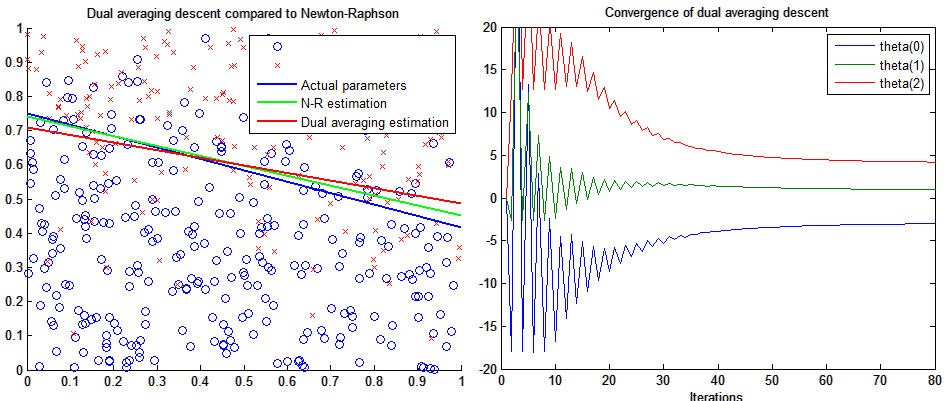
\includegraphics[width=\textwidth]{comp-vs-nr.png}\\
		 Compared to Newton-Raphson, convergence to same tolerance is much slower (258 iterations vs. 31)
	\end{frame}
	
	\begin{frame}{Single-node vs. 9-node Cycle Distributed DA}
		\centerline{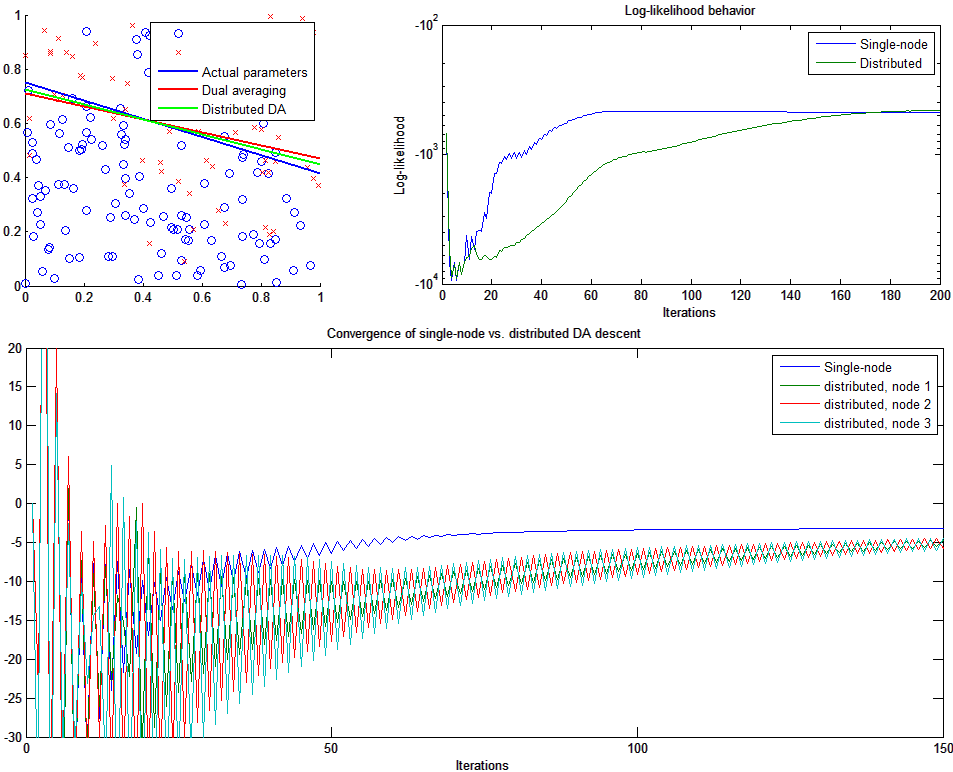
\includegraphics[width=0.75\textwidth]{singlenode-vs-dist.png}}
		Iterations required: single-node = 261, distributed = 672.
	\end{frame}
	
	\begin{frame}{Convergence of a 16-node Cycle vs. 16-node Grid}
		\centerline{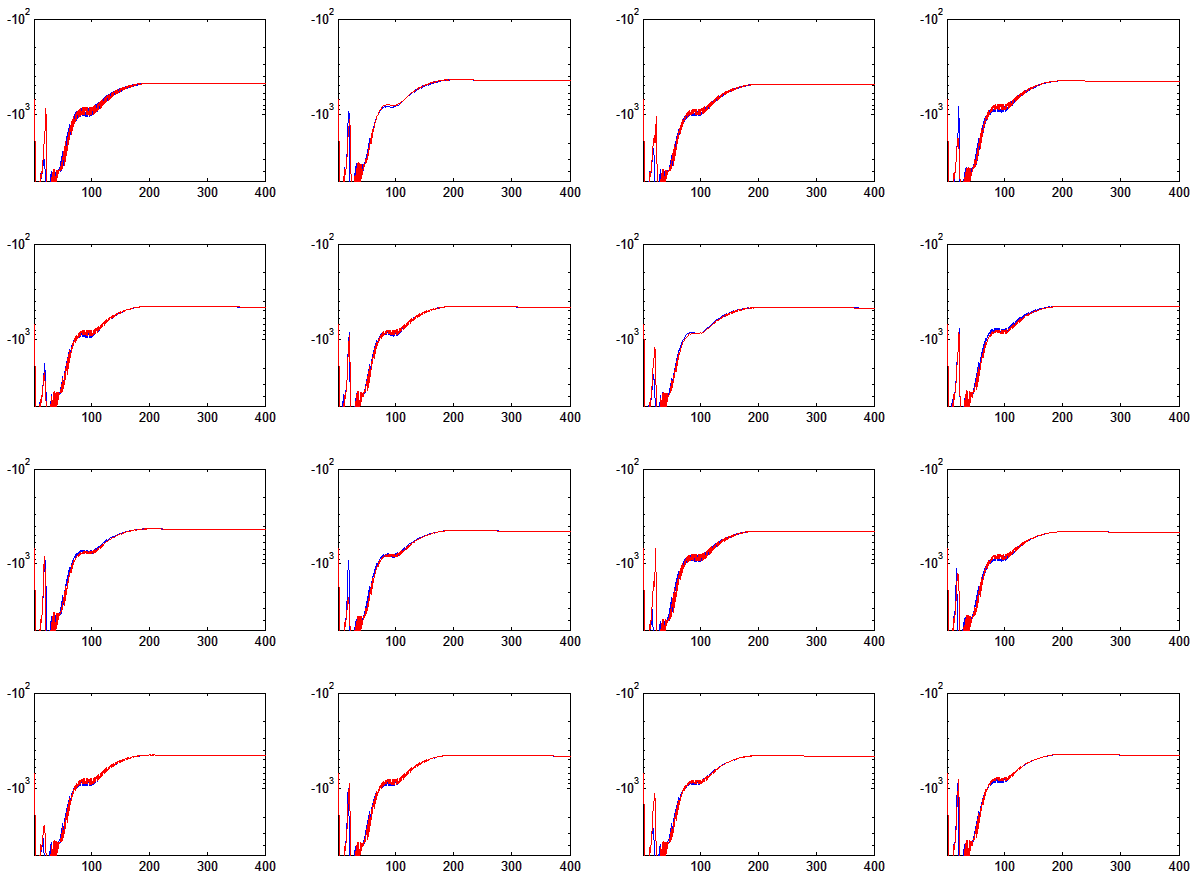
\includegraphics[width=0.75\textwidth]{grid-vs-cycle-ll-per-node.png}}
		Unexpected result: with the same weighting of the local data, convergence
		speed is almost identical even though the grid graph is twice as strongly 
		connected.
	\end{frame}
	
	\subsection{Evaluation}
	
	\section{Conclusions}
\end{document}